% UPenn Master's Thesis - PIVOT
% Based on University of Pennsylvania Ph.D. Dissertation LaTeX Template v.20221216
% Modified for Master of Science in Engineering
%-------------------------------------------
\documentclass[12pt]{report}
\usepackage{upennstyle_master}

%-------------------------------------------
% Additional packages
\usepackage[nonamebreak,numbers,sort&compress]{natbib}
\bibliographystyle{ieeetr}
\usepackage[mathcal]{eucal}

\newcommand{\argminB}{\mathop{\mathrm{arg\,min}}}
%-------------------------------------------

%%%%% PRELIMINARY PAGES %%%%%
\title{PIVOT: PHYSICS INFORMED AND VISION BASED ONLINE TUNING}
\author{Haiyue Chen}
\gradgroup{Robotics}
\date{2026}
\supervisor{Supervisor Name}
\supervisortitle{Full Faculty Title, Department}
\gradchair{Graduate Group Chairperson Name, Full Faculty Title}
\committee{Committee Member 1, Full Faculty Title and Affiliation}
\committee{Committee Member 2, Full Faculty Title and Affiliation}

\authorlegal{Haiyue Chen}

%\dedication{Write your dedication text in italics here.}

\acknowledgement{Write your acknowledgement text here.}

\abstract{Accurate dynamics models are essential for Model Predictive Control (MPC) of autonomous vehicles, yet the relationship between model architecture and closed-loop control performance remains poorly characterized. Fixed-parameter physics models require manual calibration and degrade when operating conditions change, while purely data-driven models demand large datasets and are sensitive to real-world sensor noise. This thesis presents PIVOT (Physics Informed and Vision Based Online Tuning), a framework that addresses these limitations through two contributions. First, PIVOT introduces the Learned Single-Track model (LST), which augments a nonlinear bicycle model with state-dependent multiplicative gains and additive biases predicted by a neural network. The network receives DINOv2 visual features as auxiliary input, allowing the dynamics to adapt to the current operating environment without explicit surface classification. Second, PIVOT provides a systematic comparison of seven dynamics models spanning three categories (fixed-parameter physics, physics-informed learned, and purely data-driven), all trained on identical trajectory data from a 1/5th-scale autonomous off-road race car. The evaluation comprises two stages: offline trajectory prediction on held-out data and closed-loop racing using Safe Information-Theoretic Learning MPC (SIT-LMPC). On the offline prediction task, the LST model achieves a pose loss of 0.573, reducing error by 2.2$\times$ compared to the best data-driven baseline (TCN, 1.242) and by 56\% compared to the fixed-parameter bicycle model (DST, 1.302). An ablation over input features reveals that LST maintains a pose loss of 0.514 even without visual input, while the data-driven models degrade by 1.4--2.4$\times$ under the same condition. These results indicate that the nonlinear physics structure in LST provides a strong inductive bias that improves both accuracy and robustness relative to less constrained architectures on noisy real-world data.}

%-------------------------------------------
\begin{document}

%%% Title Page (page i, no number printed)
\maketitle
\setcounter{page}{2}

%%% Dedication (optional)
%\makededication

%%% Acknowledgment (optional)
\makeacknowledgement

%%% Abstract (optional)
\makeabstract

%%% Table of Contents (mandatory for >= 50 pages)
\tableofcontents

%%% List of Tables (optional)
\clearpage \phantomsection \addcontentsline{toc}{chapter}{LIST OF TABLES} \begin{singlespacing} \listoftables \end{singlespacing}

%%% List of Illustrations (optional)
%\clearpage \phantomsection \addcontentsline{toc}{chapter}{LIST OF ILLUSTRATIONS} \begin{singlespacing} \listoffigures \end{singlespacing}

%%%%% MAIN TEXT %%%%%
\begin{mainf}

\chapter{Introduction}
\label{sec:introduction}

Model-based control strategies, particularly Model Predictive Control (MPC), have achieved widespread adoption in robotics by explicitly reasoning about future system behavior and constraints \cite{borrelli2012predictive}. Their performance, however, hinges critically on the fidelity of the underlying predictive model. With the growing availability of robot trajectory data and advances in machine learning, the choice of model architecture for learning dynamics from data has become a key design decision for high-performance model-based control \cite{hewing2020learning}.

This decision involves inherent trade-offs. Efficient parametric models, such as linear systems or fixed-parameter kinematic models, offer computational tractability and interpretability but may fail to capture complex nonlinear dynamics, especially when systems operate near performance limits \cite{rajamani2011vehicle}. More expressive architectures can better approximate true system behavior but risk overfitting, increased computational overhead, and reduced interpretability. Physics-informed approaches that leverage known structure can improve sample efficiency and generalization \cite{kabzan2019learning}, while purely data-driven methods offer maximum modeling flexibility at the cost of requiring more data and providing fewer interpretable failure modes \cite{punjani2015deep}.

Beyond model architecture, the operating context also influences dynamics. Road surface conditions, tire wear, and payload variations all alter vehicle behavior, yet conventional system identification produces a single fixed parameter set. A model that adapts its parameters to the current context, identified for example from onboard visual data, can maintain robust prediction accuracy across diverse conditions without manual re-calibration. Incorporating visual information into dynamics prediction, however, introduces a computational challenge. Sampling-based controllers such as MPPI evaluate the dynamics model thousands of times per control cycle, across $B$ candidate trajectories and $N$ horizon steps. Conditioning each evaluation on a high-dimensional visual embedding is prohibitively expensive. An effective architecture must therefore amortize visual processing by extracting context-dependent parameters once and reusing them across all rollout evaluations.

This paper addresses these challenges through a systematic empirical comparison in the autonomous racing domain, in which aggressive maneuvering at the limits of handling exposes the inadequacy of overly simplified models. Using a 1/5th-scale RC car platform, PIVOT trains and evaluates seven dynamics models spanning three categories on \emph{the same trajectory dataset}:
\begin{itemize}
    \item \textbf{Fixed-parameter physics models}: a nonlinear single-track (bicycle) model and a time-varying linear model, both with parameters identified offline.
    \item \textbf{Physics-informed learned models}: learned variants of the single-track and time-varying linear models, in which neural networks adapt the physics model parameters or system matrices as functions of the current state and action.
    \item \textbf{Purely data-driven models}: a multi-layer perceptron (MLP), a long short-term memory network (LSTM), and a temporal convolutional network (TCN), each predicting state derivatives directly from state-action data without explicit physics structure.
\end{itemize}

All seven models are trained on identical data, enabling a controlled comparison of \emph{model architecture choice} rather than data availability. The evaluation comprises two stages. First, each model is assessed on offline trajectory prediction accuracy, measuring how well the learned dynamics generalize to held-out trajectories across different operating conditions. Second, each model is integrated into a sampling-based MPC controller and evaluated in closed-loop autonomous racing, in which an iterative learning framework progressively improves lap times while maintaining safety constraints. This two-stage evaluation decouples open-loop prediction quality from closed-loop control performance, characterizing each model's strengths and limitations.

This investigation targets four objectives:
\begin{enumerate}
    \item[\textbf{O1.}] Identifying the level of model complexity necessary to capture vehicle dynamics for high-performance control at the limits of handling.
    \item[\textbf{O2.}] Evaluating whether physics-informed learned models can bridge the gap between fixed parametric models and purely data-driven representations.
    \item[\textbf{O3.}] Quantifying the advantages of physics-informed architectures in sample efficiency and generalization compared to purely data-driven approaches.
    \item[\textbf{O4.}] Characterizing the trade-off between model expressiveness and real-time control feasibility.
\end{enumerate}

The contributions of this paper are three-fold:
\begin{enumerate}
    \item Proposed a systematic comparison framework for seven dynamics models across three categories (fixed-parameter physics, physics-informed learned, and purely data-driven), all trained on the same dataset, isolating the effect of model structure on prediction and control performance.
    \item Developed and evaluated the integration of learned dynamics models within sampling-based MPC, specifically Model Predictive Path Integral (MPPI) control, and iterative learning control, specifically Safe Information-Theoretic Learning MPC (SIT-LMPC), on a physical 1/5th-scale racing platform, providing empirical grounding beyond simulation.
    \item Conducted a two-stage evaluation (offline trajectory prediction followed by closed-loop racing), yielding actionable insights into the trade-offs among model complexity, physics constraints, prediction accuracy, and real-time control performance.
\end{enumerate}


\chapter{Related Work}
\label{sec:related-work}

This chapter reviews prior work in three areas relevant to the proposed approach: model predictive control for autonomous racing (Section~\ref{sec:rw-mpc}), kinodynamics modeling (Section~\ref{sec:rw-kinodynamics}), and vision foundation models for robotics (Section~\ref{sec:rw-vision}).

\section{Model Predictive Control for Autonomous Racing}
\label{sec:rw-mpc}

Model Predictive Control (MPC) has become a dominant paradigm for autonomous racing and aggressive vehicle navigation due to its ability to handle complex nonlinear dynamics, enforce state and input constraints, and optimize multi-objective cost functions over a receding horizon \cite{borrelli2012predictive, liniger2015optimization}. Traditional nonlinear MPC formulations rely heavily on gradient-based optimization techniques, such as sequential quadratic programming or interior-point methods \cite{diehl2002real, amrit2011fast}. These methods have been widely deployed using simplified kinematic or dynamic bicycle models, offering fast local convergence for standard driving maneuvers \cite{kong2015kinematic}. However, gradient-based solvers require continuous, twice-differentiable dynamics models and are highly susceptible to local minima \cite{verschueren2021acados}. Furthermore, at the extreme limits of handling, where tire saturation causes highly nonlinear and non-convex transitions, these methods often struggle to maintain real-time feasibility and computational stability \cite{subosits2019racetrack}.

To handle model uncertainties and disturbances, robust control frameworks such as Tube-based MPC have been introduced \cite{mayne2005robust}. While Tube-based MPC provides strict constraint satisfaction by optimizing over a nominal trajectory and bounding deviations within an invariant tube \cite{villanueva2017robust}, it tends to yield overly conservative behaviors. This conservatism is counterproductive in racing scenarios where operating near the friction limits is strictly required \cite{goh2019toward}.

Consequently, sampling-based MPC methods have gained significant traction as a gradient-free alternative. Algorithms such as the Cross-Entropy Method and Model Predictive Path Integral (MPPI) control generate thousands of candidate input sequences, propagate them through forward simulation, and compute the optimal control law via cost-weighted averaging \cite{williams2017information, wagener2019online}. MPPI, rooted in stochastic optimal control and information-theoretic principles, treats the underlying dynamics model as a completely black-box simulator \cite{williams2016aggressive}. This property makes MPPI well-suited for integration with complex, discontinuous, or neural network-based dynamics models that cannot be easily linearized \cite{drews2019vision, pinneri2021sample}.

Beyond single-execution optimization, Iterative learning control paradigms have been integrated with MPC to leverage historical driving data \cite{bristow2006survey}. Learning Model Predictive Control (LMPC) constructs a safe set and a terminal value function from prior feasible trajectories, systematically driving the vehicle to reduce lap times in subsequent iterations while maintaining recursive feasibility \cite{rosolia2017learning, rosolia2019learning}. Recent literature has extended this to sampling-based domains; for instance, Safe Information-Theoretic LMPC (SIT-LMPC) combines the parallelizable, gradient-free nature of MPPI with the iterative performance improvement and safety guarantees of LMPC \cite{yin2022safe, pravitra2020information}. Nevertheless, the performance of both gradient-based and sampling-based iterative controllers remains limited by the fidelity and adaptability of the forward predictive dynamics model \cite{kabzan2019learning}.

\section{Kinodynamics Modeling}
\label{sec:rw-kinodynamics}

Accurate forward simulation of vehicle states, particularly during high-slip maneuvers, requires kinodynamics models that account for inertial effects, actuation delays, and the highly nonlinear interactions between the tires and varying road surfaces \cite{rajamani2011vehicle}. Historically, autonomous navigation relied heavily on first-principles physics models equipped with empirical tire formulations, such as the Pacejka Magic Formula or Brush tire models \cite{pacejka2012tire, svendenius2005brush}. While these analytical models offer strict physical interpretability, their core assumption relies on steady-state tire behavior and uniform surface conditions. Calibration requires exhaustive offline system identification, and the fixed parameterizations fail entirely when the vehicle encounters unmodeled suspension dynamics, aerodynamic changes, or spatially varying terrain \cite{brunner2017sim, kaufmann2020deep}.

To circumvent the limitations of analytical parameterization, data-driven alternative architectures have been widely explored \cite{hou2020data}. Early attempts utilized simple Multi-Layer Perceptrons (MLPs) to map current states and actions to state derivatives \cite{punjani2015deep}. To better capture the temporal dependencies and actuation delays inherent in mechanical systems, recurrent architectures such as Long Short-Term Memory (LSTM) networks and Temporal Convolutional Networks (TCNs) have been employed to process historical observation windows \cite{lenz2015deep, d2020recurrent}. More recently, continuous-time formulations like Neural Ordinary Differential Equations (Neural ODEs) have been proposed to model underlying physical processes more naturally, effectively decoupling the dynamics from the sampling frequency of the sensors \cite{chen2018neural, finzi2020simplifying}. Despite their expressivity, purely deep-learning-based dynamics models often suffer from compounding integration errors over long prediction horizons and demonstrate poor generalization outside of their training distribution \cite{asadi2019combating}.

To balance physical priors with the flexibility of machine learning, hybrid or gray-box modeling has emerged as a robust compromise \cite{ajgl2020gray}. In this paradigm, a nominal first-principles model captures the dominant rigid-body kinematics, while a data-driven module, such as a Gaussian Process (GP) or a residual neural network, is trained to predict the unmodeled dynamics including aerodynamic drag or transient tire slip \cite{kabzan2019learning, ostafew2016robust}. GPs provide the added benefit of bounded uncertainty estimation, which is critical for robust control, though they scale poorly with large datasets \cite{hewing2020learning}.

However, a fundamental limitation persists across conventional analytical, purely learned, and hybrid models: they are predominantly reactive, relying entirely on proprioceptive sensors such as IMUs and wheel speed encoders \cite{lee2020learning}. When traversing heterogeneous environments, proprioception-only models can only register a change in surface friction after the vehicle has already experienced slip. This inherent latency prevents the controller from executing proactive, anticipatory maneuvers before engaging a hazardous or low-friction surface.

\section{Vision Foundation Models for Robotics}
\label{sec:rw-vision}

Proactive control in unstructured environments necessitates rich exteroceptive perception capable of anticipating physical interactions before they occur \cite{corke2023robotics}. Historically, visually guided navigation systems relied on explicit feature engineering, such as using Support Vector Machines on texture descriptors, to estimate a discrete surface class or a scalar friction coefficient \cite{broggi2013terrain, stano2022terrain}. Subsequently, end-to-end behavioral cloning and task-specific convolutional neural networks sought to map raw image pixels directly to steering and throttle commands \cite{bojarski2016end, codevilla2018end}. While conceptually elegant, these end-to-end policies are notoriously difficult to debug, require massive amounts of domain-specific human demonstration data, and rarely generalize across different vehicle platforms or lighting conditions \cite{muller2018driving}.

Self-supervised Vision Foundation Models (VFMs) have transformed visual perception for robotics \cite{bommasani2021opportunities}. Models trained via contrastive learning, such as CLIP and MoCo, or masked image modeling like MAE on internet-scale datasets, have demonstrated remarkable zero-shot generalization capabilities \cite{radford2021learning, he2020momentum, he2022masked}. Among these, DINO and its successor DINOv2 have proven particularly effective for dense robotic tasks \cite{caron2021emerging, oquab2023dinov2}. Because DINOv2 is optimized via self-distillation with no explicit labels, its intermediate attention maps and patch-level embeddings naturally encode deep semantic properties of the scene, such as texture, geometry, and material composition, without collapsing into task-specific biases \cite{amir2021deep}.

In the domain of field robotics and off-road navigation, VFMs have been actively leveraged to construct visual risk networks and traversability maps \cite{frey2023locomotion}. For instance, recent works have utilized frozen foundation model features to distinguish between navigable terrain, deep mud, and obstacles without fine-tuning, vastly outperforming supervised baselines in zero-shot deployment scenarios \cite{kahn2021badgr, seo2023scenepic}. However, integrating these high-dimensional semantic representations directly into vehicle dynamics remains an open problem.

The standard approach to utilizing visual information in vehicle control has been a modular, decoupled pipeline: a vision system segments the image or classifies the terrain type, assigns a predefined friction parameter based on a lookup table, and passes this updated parameter to the MPC's physics model \cite{srinivasan2020end, nitsche2022fast}. This explicit pipeline is brittle; it discards the nuanced, high-dimensional contextual information contained in the original embedding, propagates classification errors directly to the controller, and fails when encountering out-of-vocabulary surfaces that do not fit into predefined categories \cite{maturko2022vision}.

Among available VFMs, CLIP \cite{radford2021learning} and DINOv2 \cite{oquab2023dinov2} represent two complementary paradigms. CLIP aligns visual and language representations through contrastive pre-training on image-text pairs, producing embeddings that excel at semantic category-level tasks such as zero-shot classification. DINOv2, trained via self-distillation without language supervision, yields patch-level embeddings that encode finer-grained visual properties such as texture, material, and geometry. For dynamics adaptation, where the relevant signal is surface appearance rather than semantic category, DINOv2 embeddings provide a richer and more continuous representation of the visual context.

A practical challenge remains: both CLIP and DINOv2 produce high-dimensional embeddings (typically 384--768 dimensions) that are expensive to propagate through the dynamics model at every step of a sampling-based controller. PIVOT addresses this by processing visual features through a parameter network once per control cycle, producing a compact parameter vector that the lightweight dynamics model reuses across all rollout evaluations. This architecture decouples visual perception cost from the sampling and horizon dimensions of the controller, bypasses explicit terrain classification, and allows the dynamics to adapt continuously to the current operating environment.

\chapter{Problem Formulation}
\label{sec:problem}

This chapter formulates the dynamics modeling problem considered in this work. The formulation captures environmental variability, specifies the available observations, and defines a trajectory-level predictive learning objective.

\section{System Dynamics}

Consider a discrete-time controlled dynamical system. Let $t \in \mathbb{N}$ index discrete time steps, $s_t \in \mathcal{S} \subset \mathbb{R}^{n_s}$ denote the system state, and $a_t \in \mathcal{A} \subset \mathbb{R}^{n_a}$ denote the control input.

In off-road driving scenarios, system dynamics depend not only on the current state and control input, but also on environmental factors such as terrain properties and tire--ground interaction. These factors are not directly observable and are modeled as a latent variable $c_t \in \mathcal{C}$.

The system evolves according to:
\begin{equation}
  s_{t+1} = f^*(s_t, a_t;\, c_t) + w_t, \qquad w_t \sim \mathcal{W},
  \label{eq:true-dynamics}
\end{equation}
where $f^*: \mathcal{S} \times \mathcal{A} \times \mathcal{C} \to \mathcal{S}$ is the unknown dynamics function and $w_t$ represents process noise.

Because the environmental variable $c_t$ is not directly measurable, its effect on system dynamics must be inferred indirectly. The learned models considered in this work are deterministic approximations of the underlying stochastic dynamics.

\section{Observations and Dataset}

In addition to state and control measurements, auxiliary observations are available, which provide indirect information about the latent environmental variable $c_t$. These observations may include high-dimensional sensory inputs.

An offline dataset of trajectory segments is assumed:
\begin{equation}
  \mathcal{D}_{\text{train}} =
  \left\{
  \big(s_{t:t+H}^{(i)},\, a_{t:t+H-1}^{(i)},\, \xi^{(i)}\big)
  \right\}_{i=1}^{N},
\end{equation}
where $H$ denotes the prediction horizon, and $\xi^{(i)}$ denotes context features associated with the beginning of the $i$-th trajectory segment.

Each tuple corresponds to a trajectory segment collected under a particular environmental condition. The horizon $H$ is chosen to match the rollout length used during downstream planning.

The dataset is collected from the physical system under varying environmental conditions and remains fixed for all models. Auxiliary observations are available for models that condition parameters on environmental context, but are not required by fixed-parameter baselines.

\section{Context-Conditioned Dynamics Modeling}

The objective is to learn a predictive model of the system dynamics that accounts for environmental variability.

Models of the following form are considered:
\begin{equation}
  \hat{s}_{t+1} = \hat{f}(s_t, a_t;\, \phi^{(i)}),
  \label{eq:learned-model}
\end{equation}
where $\hat{f}$ denotes a parameterized dynamics model whose structure is specified a priori, and $\phi^{(i)}$ denotes model parameters associated with the $i$-th trajectory segment.

The formulation assumes a Markovian representation, while allowing practical implementations to maintain additional internal state.

The parameter $\phi^{(i)}$ may be either constant or context-dependent. Context-dependent parameterizations allow the model to adapt to changes in the underlying environmental conditions.

To incorporate contextual information, $\phi^{(i)}$ is modeled as a function of context features:
\begin{equation}
  \phi^{(i)} = \psi(\xi^{(i)}),
\end{equation}
where $\psi$ is a mapping from context features to model parameters.

For each trajectory segment, the parameter vector $\phi^{(i)}$ is estimated once and reused across the prediction horizon.

Given a choice of $\hat{f}$, the learning problem reduces to estimating the corresponding parameters. Depending on the model class, these parameters may be directly optimized or produced by the mapping $\psi$.

\section{Learning Objective}

All models are trained to minimize trajectory-level prediction error:
\begin{equation}
  \min_{\Theta} \;
  \mathbb{E}_{(s_{t:t+H}, a_{t:t+H-1}, \xi) \sim \mathcal{D}_{\text{train}}}
  \left[
    \sum_{k=1}^{H}
    \mathcal{L}\big(
      s_{t+k},\,
      \hat{s}_{t+k}
    \big)
  \right],
\end{equation}
where $\hat{s}_{t+k}$ is obtained by rolling out the model over the prediction horizon.

The optimization variable $\Theta$ denotes the set of learnable quantities. For fixed-parameter models, $\Theta$ corresponds to model parameters. For context-conditioned models, $\Theta$ denotes the parameters of the mapping $\psi$.

This objective captures compounding prediction errors over the prediction horizon.

\section{Model Structure}

Different modeling approaches correspond to different choices of the function $\hat{f}$ and different assumptions on the structure of $\phi^{(i)}$.

Three categories of models are considered:

\begin{itemize}
\item \textbf{Fixed-parameter models:} $\phi^{(i)} \equiv \phi$ for all $i$, where $\phi$ is a constant parameter vector shared across all trajectory segments.

\item \textbf{Physics-informed models:} $\phi^{(i)}$ represents low-dimensional quantities that encode prior knowledge about system dynamics, corresponding to structured parameterizations.

\item \textbf{Purely data-driven models:} $\phi^{(i)}$ parameterizes high-capacity function approximators with minimal structural constraints, corresponding to flexible parameterizations.
\end{itemize}

This formulation enables a controlled comparison of different model structures under identical data and training conditions.

\chapter{Model Architectures}
\label{sec:models}

This chapter presents the PIVOT architecture and seven dynamics models of increasing expressiveness, all trained on $\mathcal{D}_{\text{train}}$. Section~\ref{sec:overview} describes the overall pipeline. Section~\ref{sec:visual-context} defines the visual context representation $\xi^{(i)}$. Section~\ref{sec:param-generator} details the parameter generator $\psi$. Section~\ref{sec:dynamics-models} specifies each dynamics model $\hat{f}$. Section~\ref{sec:efficient-rollout} explains the rollout design that enables real-time control. Table~\ref{tab:models} summarizes the model characteristics, and Table~\ref{tab:param-counts} reports parameter counts.

%--------------------------------------------------
\section{Overview}
\label{sec:overview}

All five learned models (LST, LTVL, MLP, LSTM, TCN) share a common two-stage architecture that separates parameter estimation from dynamics rollout:

\begin{enumerate}
  \item \textbf{Parameter estimation.} A shared parameter network $\psi$ maps context features $\xi^{(i)}$ to a compact parameter vector $\phi^{(i)}$. This mapping executes once per control cycle.
  \item \textbf{Dynamics rollout.} The dynamics model $\hat{f}$ consumes $\phi^{(i)}$ and rolls out a predicted trajectory over the $H$-step prediction horizon. The same $\phi^{(i)}$ is reused at every step within the horizon.
\end{enumerate}

The parameter network and dynamics model are trained jointly: the optimizer backpropagates a yaw-normalized L1 loss through the integrator and dynamics equations into the parameter network weights, which are the only trainable variables. The dynamics computation is fully differentiable in JAX, and optimization employs Adam with a learning rate of $10^{-3}$.

The models differ in the dimensionality of $\phi^{(i)}$ (Table~\ref{tab:param-counts}). The LST model requires only 17 outputs (9 physical parameters and 8 residual corrections) because the nonlinear bicycle dynamics handle the bulk of the prediction. The data-driven models require the parameter network to output the entire weight set of the dynamics model: 838 values for the MLP, 821 for the TCN, and 19,141 for the LSTM. Although these dynamics models are small by deep learning standards, the parameter network's output layer scales with the target dimensionality (e.g., $\approx$4.9M parameters for the LSTM output layer alone, 5.7$\times$ the shared backbone), amplifying the risk of overfitting on limited real-world data.

Two fixed-parameter baselines (DST, DTVL) bypass the parameter network entirely: their parameters are identified offline via system identification on $\mathcal{D}_{\text{train}}$, and remain constant during deployment. This controlled setup isolates the effect of model architecture on prediction accuracy and control performance.

%--------------------------------------------------
\section{Visual Context Representation}
\label{sec:visual-context}

The context feature vector $\xi^{(i)}$ encodes both visual and proprioceptive information about the current operating condition. It comprises two components.

\paragraph{Semantic visual features.}
A frozen DINOv2 ViT-S/14 backbone~\cite{oquab2024dinov2} extracts a 384-dimensional CLS token from each onboard camera image ($854 \times 480$ pixels, 30\,Hz). The image is resized to 256 pixels on the shorter side, center-cropped to $224 \times 224$, and normalized with ImageNet statistics before being passed through the network. The resulting feature vector is L2-normalized to unit norm. DINOv2 is selected for its ability to produce semantically rich representations without task-specific fine-tuning: the frozen backbone captures terrain texture, surface type, and scene geometry in a compact embedding that generalizes across visual conditions. Figure~\ref{fig:dino-features} visualizes the patch-level DINOv2 features for two scenes from the test track, illustrating how the representation distinguishes terrain regions (grass, pavement, buildings) without any task-specific supervision.

\begin{figure}[t]
  \centering
  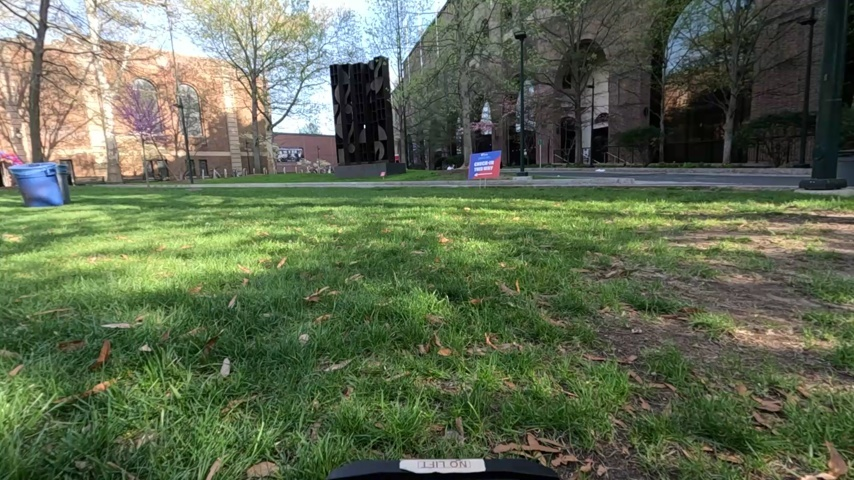
\includegraphics[height=2.6cm]{img/dino_feature/image_1776202324420642048.jpg}\kern1pt
  
\includegraphics[height=2.6cm]{img/dino_feature/image_1776202324420642048_feature.png}\hspace{0.8em}
  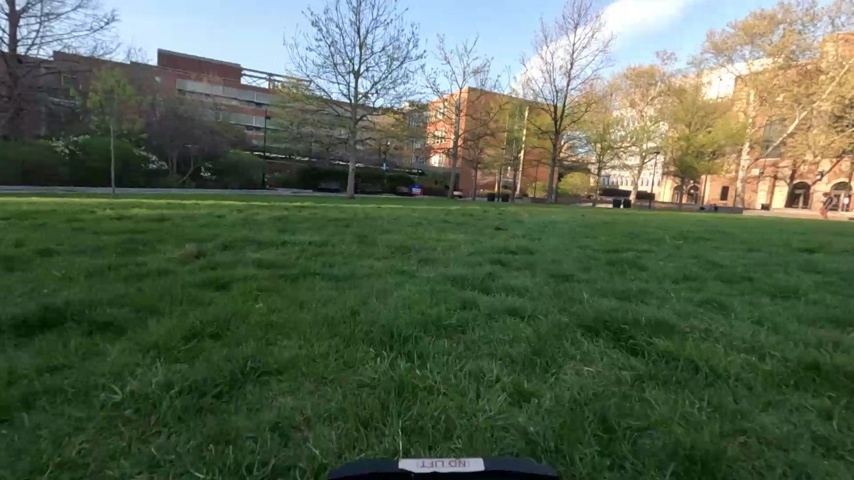
\includegraphics[height=2.6cm]{img/dino_feature/image_1776206037414451712.jpg}\kern1pt
  
\includegraphics[height=2.6cm]{img/dino_feature/image_1776206037414451712_feature.png}

  \caption{Onboard camera images (left of each pair) and corresponding DINOv2 patch-level feature visualizations (right of each pair) from two locations on the test track. Colors in the feature maps encode the NCUT spectral eigenvectors of the patch token embeddings, projected to RGB via UMAP. Semantically distinct regions (grass, pavement, buildings, sky) produce distinct feature clusters without task-specific fine-tuning}
  \label{fig:dino-features}
\end{figure}

\paragraph{State context.}
An 8-dimensional proprioceptive vector captures the vehicle's instantaneous kinematic state: body-frame velocities $(v_x, v_y, v_z)$, yaw rate $\dot{\psi}$, pitch $\theta$ and pitch rate $\dot{\theta}$, and roll $\varphi$ and roll rate $\dot{\varphi}$. These quantities are measured by the onboard IMU and GNSS system at 100\,Hz. State context provides the parameter network with information about the current dynamic regime (e.g., high-slip cornering versus straight-line driving) that is not directly visible in the camera image.

The two components are concatenated to form the context feature vector:
\begin{equation}
  \xi^{(i)} = \bigl[\,\underbrace{z_{\text{DINOv2}}}_{\text{384-dim}},\;\; \underbrace{s_{\text{ctx}}}_{\text{8-dim}}\,\bigr] \in \mathbb{R}^{392}.
  \label{eq:context-features}
\end{equation}
The DINOv2 backbone is frozen during training; only the parameter network $\psi$ is updated.

%--------------------------------------------------
\section{Parameter Generator}
\label{sec:param-generator}

The parameter generator $\psi$ maps the context feature vector $\xi^{(i)}$ to a dynamics parameter vector $\phi^{(i)} \in \mathbb{R}^{d_\phi}$, where $d_\phi$ depends on the downstream dynamics model.

\paragraph{Architecture.}
The generator is a multi-layer perceptron with PReLU activations and batch normalization between layers. It comprises two components: a shared backbone and a model-specific output stage. The backbone ($\approx$858K parameters) is identical across all five learned models, ensuring that architectural differences in downstream dynamics are not confounded by differences in feature extraction capacity.

\paragraph{Multi-head output.}
The output stage employs multiple parameter heads, each producing a candidate parameter vector. A discriminator head outputs softmax-weighted selection probabilities over the candidates. The final parameter vector is the probability-weighted average of all heads:
\begin{equation}
  \phi^{(i)} = \sum_{m=1}^{M} \alpha_m \cdot \phi^{(i)}_m, \qquad \alpha_m = \frac{\exp(d_m)}{\sum_{m'}\exp(d_{m'})},
\end{equation}
where $\phi^{(i)}_m$ denotes the $m$-th head output and $d_m$ the corresponding discriminator logit. This mixture-of-experts structure allows the network to represent multimodal parameter distributions (e.g., distinct terrain regimes) without committing to a single prediction.

\paragraph{Output scaling.}
Each predicted parameter is passed through a scaled tanh function that maps the raw network output into a physically meaningful range $[\phi_{\min}, \phi_{\max}]$:
\begin{equation}
  \phi_j = \frac{\phi_{\max,j} - \phi_{\min,j}}{2}\,\big(\tanh(x_j) + 1\big) + \phi_{\min,j}.
\end{equation}
The bounds are set based on physical plausibility (e.g., mass $> 0$, friction coefficient $\in [0, 2]$), preventing the optimizer from exploring unphysical parameter regions during training.

%--------------------------------------------------
\section{Dynamics Models}
\label{sec:dynamics-models}

Seven dynamics models are evaluated, grouped into three categories. All models predict continuous-time state derivatives that are discretized via numerical integration (Section~\ref{sec:efficient-rollout}), except as noted.

%--------------------------------------------------
\subsection{Fixed-Parameter Physics Models}
\label{sec:fixed}

These models employ conventional offline system identification with no learned components, serving as baselines.

\subsubsection{Default Single-Track Model (DST)}
\label{sec:dst}

The default single-track model is a nonlinear bicycle model with a 7-dimensional state
\begin{equation}
  s = [x,\, y,\, \delta,\, v,\, \psi,\, \dot{\psi},\, \beta]^\top,
\end{equation}
representing position $(x, y)$, steering angle $\delta$, longitudinal velocity $v$, heading $\psi$, yaw rate $\dot{\psi}$, and sideslip angle $\beta$. The two control inputs are
\begin{equation}
  a = [\dot{\delta},\, a_{\text{long}}]^\top,
\end{equation}
where $\dot{\delta}$ denotes the steering rate and $a_{\text{long}}$ the longitudinal acceleration.

The model employs a velocity-dependent switching mechanism. At low speeds ($|v| < 1.5$\,m/s), a kinematic formulation governs the dynamics. At higher speeds, a dynamic formulation with nonlinear tire force modeling becomes active. The continuous-time dynamics are discretized via fourth-order Runge--Kutta (RK4) integration with time step $\Delta t$.

The 14 physical parameters, including mass ($m = 3.74$\,kg), yaw inertia ($I_z = 0.047$\,kg$\cdot$m$^2$), front and rear cornering stiffness ($C_{Sf} = 4.72$, $C_{Sr} = 5.46$), and tire-road friction coefficient ($\mu = 1.05$), are identified offline via system identification. State constraints enforce steering limits of $\pm 0.42$\,rad, velocity bounds of $[-5, 20]$\,m/s, and steering rate limits of $\pm 3.2$\,rad/s.

\subsubsection{Default Time-Varying Linear Model (DTVL)}
\label{sec:dtvl}

The default time-varying linear model adopts a 5-dimensional state $s = [x,\, y,\, \delta,\, v,\, \psi]^\top$ with the same two control inputs. The dynamics take the form
\begin{equation}
  \dot{s} = A \begin{bmatrix} s \\ a \end{bmatrix} + B,
  \label{eq:tvl}
\end{equation}
where $A \in \mathbb{R}^{5 \times 7}$ and $B \in \mathbb{R}^{5}$ are fixed matrices identified offline. This model captures dynamics only in the vicinity of the nominal operating point around which linearization is performed, limiting its efficacy under aggressive maneuvers.

%--------------------------------------------------
\subsection{Physics-Informed Learned Models (PIVOT)}
\label{sec:physics-learned}

The two proposed PIVOT models retain known physics structure while adapting model parameters as functions of the context features $\xi^{(i)}$. By preserving established dynamics equations as an inductive bias, these architectures target improved sample efficiency and generalization compared to purely data-driven alternatives.

\subsubsection{Learned Single-Track Model (LST)}
\label{sec:lst}

The learned single-track model shares the same nonlinear bicycle dynamics and velocity-dependent switching mechanism as the DST model (Section~\ref{sec:dst}), but augments four dynamics channels with learnable corrections. Specifically, the steering rate ($\dot{\delta}$), longitudinal acceleration ($\dot{v}$), yaw acceleration ($\ddot{\psi}$), and sideslip rate ($\dot{\beta}$) channels are each modified as
\begin{equation}
  \dot{s}_j = f_{\text{physics},j}(s, a) \cdot \alpha_j + \beta_j,
  \label{eq:lst-augment}
\end{equation}
where $f_{\text{physics},j}$ denotes the original physics-based computation for the $j$-th channel, and $\alpha_j$, $\beta_j$ are learnable multiplicative gains and additive biases, respectively.

The parameter network predicts a total of 17 values from the context features:
\begin{equation}
  [\underbrace{m, I_z, l_f, l_r, h, C_{Sf}, C_{Sr}, \mu, L}_{\text{9 physical}},\;\; \underbrace{\alpha_1, \beta_1, \ldots, \alpha_4, \beta_4}_{\text{8 augmentation}}] = \psi_{\text{LST}}(\xi^{(i)}).
\end{equation}
The 9 physical parameters (mass, yaw inertia, front and rear axle distances, center-of-gravity height, front and rear cornering stiffness, friction coefficient, and vehicle length) replace the fixed values in the bicycle model equations, enabling the network to adapt tire and inertial properties to the current terrain. The 8 augmentation parameters provide residual corrections beyond what the physical parameter space can express. Gains are initialized to $\alpha_j = 1$ and biases to $\beta_j = 0$, ensuring that the model recovers the default single-track dynamics at initialization. The augmented dynamics are integrated via RK4, and the network is trained end-to-end by backpropagating through the integrator.

The LST model thus performs two complementary functions: (1) inferring terrain-dependent physical properties (e.g., reducing $\mu$ on wet grass, adjusting $C_{Sf}$ and $C_{Sr}$ for tire wear), and (2) compensating for structural model mismatch via residual corrections. The nonlinear bicycle dynamics handle the bulk of the prediction, and the network provides only calibration and residual compensation.

\subsubsection{Learned Time-Varying Linear Model (LTVL)}
\label{sec:ltvl}

The learned time-varying linear model extends the DTVL model (Section~\ref{sec:dtvl}) by replacing the fixed matrices with context-dependent ones predicted by the parameter network:
\begin{equation}
  \dot{s} = A(\xi^{(i)})\begin{bmatrix} s \\ a \end{bmatrix} + B(\xi^{(i)}),
  \label{eq:ltvl}
\end{equation}
where
\begin{equation}
  [A(\xi^{(i)}),\, B(\xi^{(i)})] = \psi_{\text{LTVL}}(\xi^{(i)}).
\end{equation}
The parameter network outputs the 40 values comprising the flattened matrix $A \in \mathbb{R}^{5 \times 7}$ and bias $B \in \mathbb{R}^{5}$. The predicted dynamics are integrated via RK4.

In contrast to the DTVL model, this formulation represents globally nonlinear dynamics through context-dependent linearization while preserving linear structure at each operating point, offering a trade-off between the interpretability of linear models and the expressiveness of nonlinear ones.

%--------------------------------------------------
\subsection{Purely Data-Driven Models}
\label{sec:data-driven}

These models learn dynamics entirely from data without explicit physics structure. All three adopt the same 5-dimensional state $s = [x,\, y,\, \delta,\, v,\, \psi]^\top$ and two control inputs as the DTVL model, and predict state derivatives $\dot{s}$ with a time step of $\Delta t = 0.05$\,s. In the PIVOT framework, the parameter network generates the entire weight set of each dynamics model, effectively functioning as a hypernetwork.

\subsubsection{Multi-Layer Perceptron (MLP)}
\label{sec:mlp}

A feedforward network with a single hidden layer of 64 units and tanh activations maps the concatenated state-action vector to state derivatives:
\begin{equation}
  \dot{s} = W_2 \tanh\!\big(\alpha\,(W_1 [s^\top, a^\top]^\top + b_1)\big) + b_2,
\end{equation}
where $\alpha$ is a learnable activation scale. The parameter network outputs all 838 weights ($W_1, b_1, W_2, b_2, \alpha$). As a memoryless model, the MLP captures instantaneous nonlinear mappings but cannot exploit temporal structure in the data.

\subsubsection{Long Short-Term Memory Network (LSTM)}
\label{sec:lstm}

The LSTM employs a single-layer cell with 64 hidden units and four standard gates (input, forget, cell candidate, and output), allowing the network to selectively retain or discard information across timesteps. The heading angle $\psi$ is represented as $[\sin\psi,\, \cos\psi]$ to avoid the discontinuity at $\pm\pi$, yielding the input vector $[\tilde{s}_t^\top, a_t^\top]^\top \in \mathbb{R}^{8}$ with $\tilde{s}_t = [x,\, y,\, \delta,\, v,\, \sin\psi,\, \cos\psi]^\top$. The LSTM cell processes this input and produces a state update via an output projection:
\begin{equation}
  h_t, c_t = \text{LSTM}(\tilde{s}_t, a_t, h_{t-1}, c_{t-1};\, \phi_{\text{LSTM}}), \qquad \Delta s_t = W_{\text{out}}\, h_t + b_{\text{out}}.
\end{equation}
Euler integration yields the next state as $s_{t+1} = s_t + \Delta s_t$, rather than the RK4 scheme employed by the other models. RK4 evaluates the dynamics function at multiple intermediate points per timestep. For a recurrent model, each intermediate evaluation advances the hidden state, causing the memory to drift from the trajectory it is meant to represent. Euler integration evaluates the LSTM cell exactly once per timestep, preserving a consistent correspondence between hidden state and trajectory history.

During training, a burn-in phase (a sequence of preceding timesteps processed without loss computation) initializes the hidden state before the loss is evaluated. The parameter network outputs all 19,141 weights comprising the gate matrices, output projection, and initial hidden and cell states.

\subsubsection{Temporal Convolutional Network (TCN)}
\label{sec:tcn}

The TCN maintains a sliding buffer of the $K = 4$ most recent state-action pairs. At each timestep, the current pair replaces the oldest entry, and the network processes the buffer through two causal 1D convolutional layers (kernel sizes 4 and 1, with a hidden dimension of 16 and tanh activations) followed by a linear output projection to state derivatives:
\begin{equation}
  \dot{s}_t = W_{\text{out}}\, \text{Conv}_2\!\big(\tanh(\text{Conv}_1(\text{buf}_t))\big) + b_{\text{out}}.
\end{equation}

Unlike the LSTM, the TCN can employ RK4 integration because its buffer remains fixed during the intermediate sub-steps of each timestep: only the final integrated state updates the buffer for the next step. This avoids the hidden-state drift that prevents the LSTM from employing higher-order integrators. The parameter network outputs all 821 weights comprising the convolutional kernels and output projection.

%--------------------------------------------------
\section{Efficient Rollout Design}
\label{sec:efficient-rollout}

Deploying learned dynamics within a sampling-based controller such as MPPI imposes strict computational constraints. At each control cycle, MPPI samples $K$ candidate control sequences and rolls out each through the dynamics model over the $H$-step horizon. A naive implementation that invokes the parameter network at every step of every sample incurs $K \times H$ forward passes.

The two-stage architecture eliminates this bottleneck. The parameter network executes once per control cycle, producing a single parameter vector $\phi^{(i)}$ from the current context features. The dynamics model then rolls out all $K$ candidate trajectories using the same $\phi^{(i)}$. This factorization reduces the parameter network cost from $O(K \cdot H)$ to $O(1)$ per control cycle.

\paragraph{Vectorized rollout.}
The dynamics computation is implemented in JAX, enabling vectorized rollout of all $K$ trajectories in parallel via \texttt{jax.vmap}. Because each trajectory shares the same parameter vector, the rollout reduces to a batched scan over timesteps with no per-sample branching.

\paragraph{Numerical integration.}
Continuous-time state derivatives are discretized via fourth-order Runge--Kutta (RK4) integration for all models except the LSTM, which employs Euler integration to preserve hidden-state consistency (Section~\ref{sec:lstm}). The TCN employs RK4 with its temporal buffer held fixed during sub-steps. A configurable sub-stepping ratio allows finer integration resolution without changing the control timestep.

\paragraph{Computational cost.}
The parameter network ($\approx$858K parameters) adds negligible overhead relative to the rollout computation. For the LST model with $K = 512$ samples and $H = 9$ steps, the complete control cycle (parameter prediction and trajectory rollout) executes within the real-time budget of a 50\,Hz control loop, occupying less than 3\% of the 20\,ms cycle on an NVIDIA RTX A6000. The dominant cost is the dynamics rollout itself, not the parameter network, confirming that the two-stage factorization achieves its design goal.

%--------------------------------------------------
\begin{table}[t]
\centering
\caption{Summary of the seven dynamics models evaluated in this work. LST and LTVL are the proposed PIVOT models; the remaining five serve as baselines. Physics-informed models retain known dynamics equations, while data-driven models learn the full state-derivative mapping from data. Temporal models incorporate past state-action history.}
\label{tab:models}
\small
\begin{tabular}{@{}llcccc@{}}
\toprule
Category & Model & Dim. & Learned & Physics & Temporal \\
\midrule
\multirow{2}{*}{Fixed} & DST & 7 & -- & \checkmark & -- \\
 & DTVL & 5 & -- & \checkmark & -- \\
\midrule
\multirow{2}{*}{PIVOT} & LST & 7 & \checkmark & \checkmark & -- \\
 & LTVL & 5 & \checkmark & \checkmark & -- \\
\midrule
\multirow{3}{*}{Data-Driven} & MLP & 5 & \checkmark & -- & -- \\
 & LSTM & 5 & \checkmark & -- & \checkmark \\
 & TCN & 5 & \checkmark & -- & \checkmark \\
\bottomrule
\end{tabular}
\end{table}

\begin{table}[t]
\centering
\caption{Parameter counts for each learned model. All models share the same 858K-parameter backbone; the output layer scales with the number of predicted dynamics parameters. The LST model requires only 17 outputs, keeping total parameters near the backbone size, while the LSTM requires 19,141 outputs, inflating the total to 5.8M and increasing overfitting risk.}
\label{tab:param-counts}
\small
\begin{tabular}{@{}lrrr@{}}
\toprule
Model & Dynamics Params & Output Layer & Total \\
\midrule
LST & 17 & 4,369 & 862,225 \\
LTVL & 40 & 10,280 & 868,136 \\
MLP & 838 & 215,366 & 1,073,222 \\
TCN & 821 & 210,997 & 1,068,853 \\
LSTM & 19,141 & 4,919,237 & 5,777,093 \\
\bottomrule
\end{tabular}
\end{table}


\chapter{Control and Evaluation Framework}
\label{sec:control}

All seven dynamics models are integrated into a unified control framework for evaluation. This chapter describes the sampling-based MPC controller employed for trajectory optimization (Section~\ref{sec:mppi}) and the iterative learning framework adopted for closed-loop evaluation (Section~\ref{sec:sitlmpc}).

\section{Sampling-Based MPC (MPPI)}
\label{sec:mppi}

All models are integrated into an MPPI controller, a sampling-based MPC method that accommodates nonlinear dynamics and constraints without requiring gradients of the dynamics model.

At each time step $t$, MPPI samples $K$ candidate control sequences $\{a^{(k)}_{t:t+H}\}_{k=1}^K$ from a distribution centered around the previous optimal sequence. Each candidate sequence is rolled out using the current dynamics model $\hat{f}$ to obtain predicted trajectories $\{\hat{s}^{(k)}_{t:t+H}\}_{k=1}^K$. Trajectories are scored via a cost function that combines tracking error, control effort, and constraint violations:
\begin{equation}
  J^{(k)} = \sum_{j=0}^{H} c(\hat{s}^{(k)}_{t+j},\, a^{(k)}_{t+j}) + \lambda \max\!\big(0,\, g(\hat{s}^{(k)}_{t+j})\big),
\end{equation}
where $c$ penalizes deviation from a reference path and excessive control magnitude, and $g$ encodes safety constraints such as track boundaries. The final control is computed as a cost-weighted average:
\begin{equation}
  a_t = \sum_{k=1}^K w^{(k)} a^{(k)}_t, \qquad w^{(k)} = \frac{\exp(-\gamma\, J^{(k)})}{\sum_{k'} \exp(-\gamma\, J^{(k')})},
\end{equation}
where $\gamma$ is a temperature parameter governing the sharpness of the weighting.

Because MPPI requires only forward simulation of the dynamics model, it is compatible with all seven model architectures without modification. The fidelity of the dynamics model directly determines the quality of the sampled trajectory predictions and, consequently, the resulting control performance.

\section{Safe Information-Theoretic Learning MPC (SIT-LMPC)}
\label{sec:sitlmpc}

To evaluate long-term learning performance, SIT-LMPC is adopted as a framework for safe iterative improvement. SIT-LMPC combines sampling-based optimization with iterative learning to progressively reduce lap times while maintaining safety through learned value functions from previous iterations.

For every time step $k \in \overline{\mathbb{Z}}_{+}$, let $x^{l}(k)$, $u^{l}(k)$, and $w^{l}(k)$ denote the system state, control input, and stochastic disturbance at the $l$-th iteration. An iteration $l$ is \textit{feasible} if $x^{l}(k) \in \mathcal{X}$ and $u^{l}(k) \in \mathcal{U}$ for all $k \in \overline{\mathbb{Z}}_{+}$, and $\lim_{k \rightarrow \infty} x^{l}(k) \in \mathcal{T}$, the target set.

Let $\mathcal{I}^l \triangleq \{ i \in [0, l] : \text{iteration } i \text{ is feasible}\}$ denote the set of indices of feasible iterations up to iteration $l$. The \textit{sampled safe set} $\mathcal{S}^l$ at iteration $l$ is formulated as
\begin{equation}
  \mathcal{S}^{l} \triangleq \left\{x^{i}(k) :\;  i \in \mathcal{I}^{l},\; k \in \overline{\mathbb{Z}}_{+} \right\},
\end{equation}
consisting of all states along feasible trajectories up to iteration $l$. The convex hull $\mathcal{CS}^l$ of $\mathcal{S}^l$ serves as a terminal constraint set.

The $l$-th iteration cost is $J^{l}(x_0, u^{l}(\cdot)) \triangleq \sum_{k=0}^{\infty} h(x^{l}(k), u^{l}(k))$, and the $l$-th iteration value function is $V^l(x_0) \triangleq \mathbb{E}[J^{l}(x_0, u^{l}(\cdot))]$, which serves as the terminal cost.

At each iteration $l$ and time $t$, SIT-LMPC solves the constrained finite-time optimal control problem:
\begin{subequations}
\label{eq:sitlmpc}
\begin{align}
  J_{\text{LMPC}}^{l}(x^{l}(t)) &\triangleq \min_{u^{l}_{\cdot \mid t}} \mathbb{E}\!\left[\sum_{k=t}^{t+T-1} h(x^{l}_{k \mid t},\, u^{l}_{k \mid t}) + V^{l}(x^{l}_{t+T \mid t})\right] \\
  \text{s.t.} \quad & x^{l}_{k+1 \mid t} = f(x^{l}_{k \mid t},\, u^{l}_{k \mid t},\, w^{l}(k)), \quad k \in \{t, \ldots, t+T-1\} \\
  & x^{l}_{t \mid t} \stackrel{\text{a.s.}}{=} x^{l}(t), \\
  & x^{l}_{k \mid t} \in \mathcal{X},\quad u^{l}_{k \mid t} \in \mathcal{U} \quad \text{a.s.}, \quad k \in \{t, \ldots, t+T-1\}, \\
  & x^{l}_{t+T \mid t} \in \mathcal{CS}^{l-1} \quad \text{a.s.},
\end{align}
\end{subequations}
where $x^{l}_{k \mid t}$ and $u^{l}_{k \mid t}$ denote predicted states and inputs given measurement $x^{l}(t)$. The terminal constraint $x^{l}_{t+T \mid t} \in \mathcal{CS}^{l-1}$ enforces safety by requiring the predicted trajectory to terminate within the convex hull of previously demonstrated safe states.

\paragraph{Integration with Learned Models.}
Each of the seven dynamics models provides the forward prediction function $f$ in the SIT-LMPC formulation~\eqref{eq:sitlmpc}. The models are trained offline on $\mathcal{D}_{\text{train}}$ and deployed for online prediction without further adaptation. At each control cycle, the controller queries the dynamics model with the current state and candidate actions, rolls out trajectories utilizing the model, applies the terminal constraint derived from the learned safe set, and computes the cost-weighted optimal control. The models remain fixed during deployment, testing the robustness and generalization of each architecture from offline training data to online control under constrained real-time conditions.


\chapter{Experiments}
\label{sec:experiments}

This chapter evaluates the seven dynamics models described in Chapter~\ref{sec:models}. Section~\ref{sec:hardware} details the hardware platform and data collection procedure. Section~\ref{sec:offline} assesses offline trajectory prediction accuracy on held-out data, and Section~\ref{sec:closedloop} evaluates closed-loop control performance in autonomous racing utilizing the SIT-LMPC framework (Section~\ref{sec:sitlmpc}).

\section{Hardware Setup and Data Collection}
\label{sec:hardware}

\subsection{Platform}
\label{sec:platform}
All experiments are conducted on a 1/5th-scale autonomous off-road race car equipped with three primary subsystems:
\begin{itemize}
    \item An NVIDIA Jetson Orin AGX for onboard computing.
    \item A Fixposition Vision-RTK 2 GNSS system for state estimation and localization.
    \item Motor and steering servo interfaces for actuation.
\end{itemize}
A GoPro camera mounted on the vehicle captures onboard RGB images at $854 \times 480$ resolution and approximately 30\,Hz for visual feature extraction. State estimation is performed using an Extended Kalman Filter that fuses IMU measurements and encoder data. The vehicle operates on a closed-loop track in an outdoor grassy environment, in which natural terrain variations introduce surface variability that affects tire--road interaction and vehicle dynamics. The nominal platform parameters are listed in Table~\ref{tab:params}.

\begin{table}[h]
\centering
\caption{Nominal Parameters of the 1/5th-Scale RC Car Platform}
\label{tab:params}
\begin{tabular}{lcc}
\toprule
\textbf{Parameter} & \textbf{Symbol} & \textbf{Nominal Value} \\
\midrule
Vehicle length & $l$ & 0.531\,m \\
Total vehicle mass & $m$ & 15.32\,kg \\
Moment of inertia (z-axis) & $I_z$ & 0.643\,kg$\cdot$m$^2$ \\
Distance to front axle & $l_f$ & 0.2725\,m \\
Distance to rear axle & $l_r$ & 0.2585\,m \\
Center-of-gravity height & $h_{\text{cg}}$ & 0.1825\,m \\
Front cornering stiffness & $C_{S,f}$ & 5.3507\,N/rad \\
Rear cornering stiffness & $C_{S,r}$ & 5.3507\,N/rad \\
Friction coefficient & $\mu$ & 0.8 \\
\bottomrule
\end{tabular}
\end{table}

\subsection{Data Collection}
\label{sec:datacollection}

The training dataset $\mathcal{D}_{\text{train}}$ is collected through a two-step procedure. First, a human operator manually drives the vehicle around the track to generate a set of reference waypoints that define the racing line. Second, an MPPI controller tracks these waypoints at varying reference speeds, and the resulting trajectories are recorded. Multiple runs at different speeds ensure that the dataset covers a broad range of operating conditions, from moderate cruising to aggressive cornering near the limits of handling.

Each recorded trajectory comprises three synchronized data streams:
\begin{itemize}
    \item \textbf{State log} (100\,Hz): At each timestep, 21 fields are recorded, including position $(x, y, z)$, longitudinal and lateral velocities $(v_x, v_y)$, orientation (yaw $\psi$, pitch, roll), angular rates (yaw rate $\dot{\psi}$, pitch rate, roll rate), steering angle $\delta$, sideslip angle $\beta$, and the applied control inputs (steering angle velocity $\dot{\delta}$ and longitudinal acceleration $a_{\text{long}}$). The planned reference coordinates from the MPPI controller are also stored for each timestep.
    \item \textbf{Image log} (30\,Hz): Each GoPro frame is stored as a timestamped JPEG image and associated with pre-extracted visual features. The feature vector consists of a 384-dimensional semantic embedding from DINOv2 and a 3-dimensional low-level descriptor (mean RGB values), yielding a 387-dimensional representation per frame.
    \item \textbf{Image feature database}: The DINOv2 semantic features and low-level RGB features are pre-computed offline and stored alongside each image timestamp, enabling efficient retrieval during training and evaluation without repeated forward passes through the vision backbone.
\end{itemize}

The state log and image log are synchronized via nanosecond-precision timestamps. All seven dynamics models are trained on the state log portion of this identical dataset. The DINOv2 image features are additionally utilized as input to the learned models in the \emph{full} feature mode, providing visual information about the current operating environment.

\section{Offline Trajectory Prediction}
\label{sec:offline}

The training set contains 11,810 samples (106,290 state transitions).

\subsection{Evaluation Protocol and Metrics}

Each sample consists of an initial 7-dimensional state $s_0$, paired with the corresponding DINOv2 and state-context features, and a control sequence of length $N = 9$. The model autoregressively rolls out predicted states $\hat{s}_{1:N}$ from $s_0$, and the resulting 9-step trajectory is compared against the ground-truth states $s_{1:N}$.

The evaluation partitions the dataset into training, validation, and test sets based on waypoint trajectories: each split contains trajectories generated from entirely distinct sets of reference waypoints, ensuring that no waypoint sequence appears in more than one split. This trajectory-level partitioning prevents data leakage from overlapping spatial regions and provides a strict test of generalization to unseen driving lines. The training set serves for model fitting, the validation set for early stopping and hyperparameter selection, and the test set for final reporting. All models share identical splits.

Prediction quality is measured using a \emph{yaw-normalized L1 loss}. For non-angular state components (position $x$, $y$, steering angle $\delta$, and velocity $v$), the metric computes the L1 error summed over the prediction horizon. For the heading angle $\psi$, the angular difference is wrapped to $[-\pi, \pi]$ via $\text{arctan2}(\sin(\hat{\psi} - \psi),\, \cos(\hat{\psi} - \psi))$ before taking the absolute value, mitigating artificial penalties from angle wraparound. This loss is reported both per state dimension ($\mathcal{L}_x$, $\mathcal{L}_y$, $\mathcal{L}_\psi$, $\mathcal{L}_v$) and as an aggregate \emph{pose loss} averaging over position and heading components.

In addition to individual model performance, three \emph{feature modes} are compared to assess the contribution of visual context:
\begin{itemize}
    \item \textbf{Full}: the network receives both image features (DINOv2 embeddings) and state context as input.
    \item \textbf{State contexts only}: the network receives only state context, without image features.
    \item \textbf{Default}: fixed parameters identified offline, with no learned adaptation.
\end{itemize}

\subsection{Results}

Table~\ref{tab:offline-results} summarizes the test-set prediction loss for all models. Three findings emerge from these results.

\paragraph{Physics-informed models outperform purely data-driven approaches on real-world data.}
Among all models evaluated in \emph{full} feature mode, the LST model achieves the lowest test pose loss, outperforming the best data-driven baseline (TCN) by 2.2$\times$ (Table~\ref{tab:offline-results}). The data-driven models exhibit higher errors despite greater representational flexibility. Trajectory data from physical systems contains noise from sensor error, actuator delay, and environmental disturbances. Without structural constraints, data-driven models must jointly learn the dynamics and absorb the noise distribution from a limited dataset, leading to overfitting. The Gap column in Table~\ref{tab:offline-results} quantifies this: data-driven models exhibit train-test gaps of 1.9--2.3$\times$, while the LST model maintains the smallest gap (1.6$\times$). As discussed in Table~\ref{tab:param-counts}, this difference traces to the output dimensionality of the parameter network. The LST output layer contains $\approx$2K parameters, while the LSTM output layer inflates to $\approx$4.9M, providing capacity to memorize training trajectories but not to generalize. The physics structure in LST acts as a regularizer: it reduces the output space from thousands of unconstrained weights to 8 physically interpretable corrections.

The validation column further illustrates this. For the LST model, validation loss closely tracks training loss, indicating stable learning. The data-driven models show increasing train-val divergence that early stopping does not fully resolve, as the held-out test losses confirm.

\paragraph{Nonlinear physics structure provides a stronger inductive bias than linear structure.}
Although both PIVOT models leverage physics-based priors, the LST model reduces pose loss by 69\% relative to the LTVL model. The per-dimension breakdown (Table~\ref{tab:offline-results}) reveals the source: the LTVL model attains competitive heading error but suffers from large position errors. This disparity arises because the LTVL must approximate nonlinear dynamics through state-dependent linear matrices, constraining each local approximation to a linear manifold. At the limits of handling, where tire forces saturate and lateral-longitudinal coupling becomes highly nonlinear, this linear structure is insufficient. The LST model retains the full nonlinear tire force model and switching mechanism, requiring the network to learn only multiplicative and additive corrections rather than the entire nonlinear mapping.

The fixed-parameter baselines perform considerably worse than all learned models (Table~\ref{tab:offline-results}), confirming the benefit of data-driven adaptation. The per-dimension results (Table~\ref{tab:offline-results}) show that the DST-default model fails particularly on velocity prediction, indicating that fixed offline identification cannot capture speed-dependent dynamics across diverse operating conditions.

\paragraph{Physics structure mitigates dependence on visual features.}
The state-only ablation in Table~\ref{tab:offline-results} reveals the role of visual context in model robustness. The LST model without image features maintains nearly the same test pose loss as the full-feature variant, indicating that the physics-based inductive bias compensates for missing visual information. The LTVL and data-driven models, in contrast, degrade sharply without visual input. This pattern connects to the architectural analysis: the data-driven parameter networks must generate hundreds to thousands of dynamics weights from the input features, creating a high-dimensional output space that can latch onto spurious feature correlations. When those features are removed, the learned mapping collapses. The LST parameter network outputs only 8 values, and the bicycle dynamics handle the remainder of the prediction, leaving little room to overfit to any particular input modality.

\begin{table}[t]
\centering
\caption{Offline trajectory prediction results ($N = 9$ step horizon, lower is better). Pose loss is reported across train/val/test splits; the Gap column (test/train ratio) quantifies generalization. Per-dimension test losses reveal which state components each model struggles with. The LST model achieves the lowest test loss, the smallest generalization gap, and robust performance even without visual features.}
\label{tab:offline-results}
\small
\begin{tabular}{@{}llccccccccc@{}}
\toprule
 & & \multicolumn{4}{c}{Pose Loss} & \multicolumn{4}{c}{Test Loss by State Dimension} \\
\cmidrule(lr){3-6} \cmidrule(l){7-10}
Model & Features & Train & Val & Test & Gap & $x$ & $y$ & $\psi$ & $v$ \\
\midrule
DST & default & 1.57 & 0.82 & 1.30 & -- & 1.23 & 1.19 & 1.49 & 10.01 \\
DTVL & default & 4.02 & 2.80 & 3.75 & -- & 4.54 & 5.22 & 1.48 & 1.58 \\
\midrule
LST & full & 0.36 & 0.42 & \textbf{0.57} & 1.6 & \textbf{0.43} & \textbf{0.40} & 0.89 & \textbf{1.03} \\
LTVL & full & 0.62 & 0.95 & 1.86 & 3.0 & 2.23 & 2.20 & 1.16 & 1.03 \\
MLP & full & 0.71 & 0.77 & 1.32 & 1.9 & 1.57 & 1.59 & \textbf{0.81} & 1.35 \\
LSTM & full & 0.68 & 1.10 & 1.39 & 2.0 & 1.09 & 1.53 & 1.54 & 1.21 \\
TCN & full & 0.53 & 0.86 & 1.24 & 2.3 & 1.31 & 1.47 & 0.95 & 1.23 \\
\midrule
LST & state & 0.39 & 0.40 & \textbf{0.51} & 1.3 & 0.40 & 0.38 & 0.77 & 1.06 \\
LTVL & state & 6.65 & 6.71 & 8.16 & 1.2 & 3.82 & 6.46 & 14.19 & 6.25 \\
MLP & state & 1.77 & 1.55 & 2.58 & 1.5 & 3.18 & 3.77 & 0.79 & 1.34 \\
LSTM & state & 2.74 & 2.38 & 3.27 & 1.2 & 3.63 & 4.50 & 1.69 & 1.57 \\
TCN & state & 2.07 & 1.60 & 2.60 & 1.3 & 3.13 & 3.87 & 0.79 & 1.34 \\
\bottomrule
\end{tabular}
\end{table}

\section{Computational Cost}
\label{sec:compute}

To address \textbf{O4}, the inference latency of each model is profiled on an NVIDIA RTX A6000 GPU (48\,GB VRAM, CUDA Compute Capability 8.6) with an AMD EPYC 7452 CPU running Ubuntu 22.04. All models are JIT-compiled via JAX prior to measurement. The PIVOT inference pipeline consists of three stages: DINOv2 feature extraction, parameter network forward pass, and dynamics rollout over the 9-step prediction horizon. DINOv2 feature extraction requires 4,553\,$\mu$s per image but runs as an asynchronous process at the camera frame rate (30\,Hz), placing it outside the control-loop critical path. The parameter network forward pass adds 91--113\,$\mu$s ($B = 1$) and is comparable across all models. The dynamics rollout, reported in Table~\ref{tab:latency}, constitutes the primary differentiator and the dominant cost on the critical path.

For an MPPI controller sampling $B = 512$ candidate trajectories, the control-loop cost (parameter network + rollout) is approximately 96 + 477 = 573\,$\mu$s for the LST model. At a 50\,Hz control rate (20\,ms budget), this occupies less than 3\% of the cycle, leaving ample margin for cost evaluation, constraint checking, and communication.

Table~\ref{tab:latency} compares this PIVOT architecture against a hypothetical alternative in which a single large network directly maps from state, control, and DINOv2 features to state derivatives at each rollout step (399-dimensional input per step, processed $B \times 9$ times per control cycle). At $B = 512$, the direct approach requires 732--914\,$\mu$s, roughly 1.5--2.0$\times$ the PIVOT pipeline (267--477\,$\mu$s rollout). At $B = 1024$, the gap widens further (1,158--1,343\,$\mu$s vs.\ 334--545\,$\mu$s). The PIVOT architecture avoids this cost by invoking the parameter network once per control cycle, producing a compact parameter vector that the lightweight dynamics model then reuses across all $B \times 9$ rollout steps. The direct approach must propagate the full 399-dimensional feature vector through every step of every sample, incurring overhead that grows linearly with both batch size and horizon length.

\begin{table}[t]
\centering
\caption{Control-loop latency ($\mu$s): PIVOT (parameter network invoked once, then lightweight dynamics rollout) vs.\ a direct approach (large network at every rollout step with 399-dim input). PIVOT rollouts operate on 17--1,717 parameters per step; direct rollouts propagate 357K--738K parameters per step. All values averaged over 5,000 JIT-compiled calls on an NVIDIA RTX A6000.}
\label{tab:latency}
\small
\begin{tabular}{@{}lrrccccc@{}}
\toprule
 & & & \multicolumn{5}{c}{Latency ($\mu$s)} \\
\cmidrule(l){4-8}
Model & Total & Rollout & $B$=1 & $B$=64 & $B$=256 & $B$=512 & $B$=1024 \\
\midrule
\multicolumn{8}{l}{\textit{PIVOT (param.\ net runs 1$\times$, dynamics runs $B \times 9\times$)}} \\
LST & 860K & 17 & 484 & 469 & 472 & 477 & 515 \\
LTVL & 868K & 40 & 253 & 328 & 336 & 347 & 334 \\
MLP & 1.07M & 838 & 288 & 284 & 310 & 330 & 401 \\
LSTM & 5.78M & 1,717 & 299 & 220 & 217 & 267 & 409 \\
TCN & 1.07M & 821 & 417 & 433 & 446 & 469 & 545 \\
\midrule
\multicolumn{8}{l}{\textit{Direct (all params in rollout, runs $B \times 9\times$)}} \\
LST & 631K & 631K & 304 & 553 & 686 & 914 & 1,343 \\
LTVL & 635K & 635K & 303 & 556 & 705 & 912 & 1,306 \\
MLP & 738K & 738K & 297 & 550 & 735 & 828 & 1,250 \\
LSTM & 357K & 357K & 279 & 491 & 602 & 732 & 1,158 \\
TCN & 735K & 735K & 298 & 592 & 862 & 839 & 1,271 \\
\bottomrule
\end{tabular}
\end{table}

\section{Closed-Loop Control}
\label{sec:closedloop}


\input{sections/conclusion}

\end{mainf}

%%%%% BIBLIOGRAPHY %%%%%
\begin{bibliof}
\bibliography{bibliography}
\end{bibliof}

\end{document}
